\section{\uppercase{Building the Minimap Representation}}
\label{sec:encoding}

\noindent
To vary the information encoded in each minimap, we first reconstruct the visible trace. We then map individual pen signals to color and combine them without changing the trajectory or rendering geometry.

\subsection{The Visible Trace}
\noindent
Let $q_i=(x_i,y_i,t_i,s_i,z_i,a_i,p_i)$, $i=1,\dots,N$, be the samples of a handwriting task recording, where $x_i$ and $y_i$ are the spatial coordinates of sample $i$, $t_i$ is its timestamp, $s_i$ indicates surface contact, $z_i$ is the azimuth, $a_i$ the altitude and $p_i$ the pen pressure.

The static image uses only position and the contact indicator: a segment between samples $i$ and $i+1$ is drawn if both are on the surface, that is, if $i\in\mathcal{S}=\{i:s_i=1\ \mathrm{and}\ s_{i+1}=1\}$. This preserves pen lifts as gaps instead of joining the end of one stroke to the beginning of the next, and neither the in-air trajectory nor the duration of a lift appears in the image. Contact points alone determine the bounding box, which is centered on a $512\times512$ white canvas with a 20-pixel margin, using one scale factor for both axes. Segments are drawn in RGB $(30,30,30)$ with constant 4-pixel thickness, rendered at three times the target resolution and reduced with Lanczos filtering.

Fitting every record to its own canvas removes absolute size: geometrically similar samples of different sizes produce the same image.

\subsection{Adding One Signal}
\begin{figure}[t]
\centering
\setlength{\unitlength}{\columnwidth}
\begin{picture}(1,0.401)
\put(0.12,0){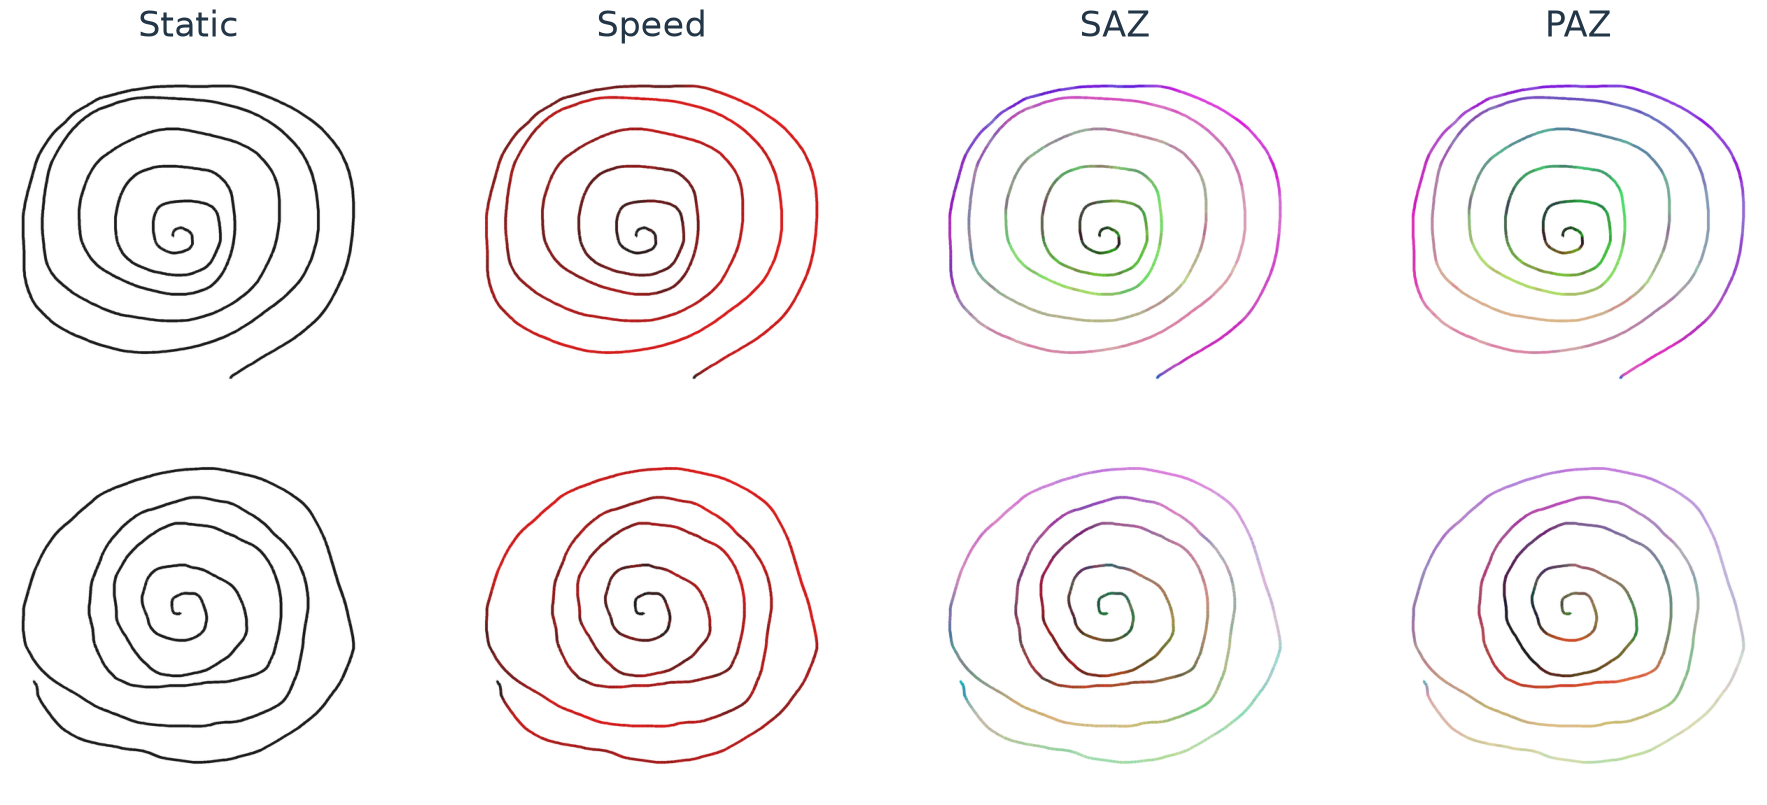
\includegraphics[width=0.88\columnwidth]{progressive_encoding_nolabels.png}}
\put(0.065,0.301){\makebox(0,0){\rotatebox{90}{\footnotesize Healthy}}}
\put(0.065,0.100){\makebox(0,0){\rotatebox{90}{\footnotesize PD}}}
\end{picture}
\caption{Building a pseudodynamic minimap from the same spiral trace. Rows show one healthy and one PD example, selected by a fixed identifier rule. Columns move from the static trace (encoding~1 in Table~\ref{tab:encoding}) to speed alone (2) and two RGB triplets, $SAZ$ (8) and $PAZ$ (9). The trajectory is unchanged; color describes within-recording variation.}
\label{fig:progressive}
\end{figure}
\noindent
Four measurements are candidates for color: speed ($S$), pressure ($P$), altitude ($A$) and azimuth ($Z$). Altitude describes pen inclination relative to the surface, while azimuth describes its orientation in the tablet plane. We first encode each signal alone (encodings 2--5 in Table~\ref{tab:encoding}), always in the red channel, with green and blue fixed at 30.

For a surface segment, speed is calculated directly from the consecutive coordinates and timestamps:
\begin{equation}
 v_i=\frac{\sqrt{(x_{i+1}-x_i)^2+(y_{i+1}-y_i)^2}}{t_{i+1}-t_i}.
 \label{eq:speed}
\end{equation}
We use $\log(1+v_i)$ in native tablet units, which compresses large values before the intensity mapping; pressure and altitude use the arithmetic mean of the two endpoint measurements. Azimuth requires a circular reference: we convert the recorded tenths of a degree to radians, compute the mean direction over contact samples, and center each angle on that direction, wrapping it into $[-\pi,\pi]$ before the endpoint average is taken. This reduces the effect of an arbitrary zero-degree boundary.

Each transformed signal $f_i$ is scaled within the recording being rendered. Let $q_{.05}$ and $q_{.95}$ be its fifth and ninety-fifth percentiles over surface segments. The channel value is
\begin{equation}
 c_i=\operatorname{round}\!\left(30+190\operatorname{clip}\!\left(\frac{f_i-q_{.05}}{q_{.95}-q_{.05}},0,1\right)\right),
 \label{eq:color}
\end{equation}
The white background stays outside the semantic range. Each record is normalized independently, without a cohort-wide reference distribution or class labels, so color describes relative variation within a recording: the same red value in two images need not represent the same absolute speed or pressure, and circular centering likewise removes absolute pen orientation.

\subsection{Combining Signals in RGB}
\noindent
We assign one scalar signal to each RGB channel and evaluate all four subsets of size three (encodings 6--9). Table~\ref{tab:encoding} numbers the nine encodings used throughout the paper, and Figure~\ref{fig:progressive} illustrates the progression; all combinations use the same geometry, background and rendering settings as the static and single-signal images. In an $SAZ$ spiral, speed is lowest near the center and rises along the outer turns, while altitude and azimuth vary over different portions of the trajectory, so the RGB image places all three variations on the same stroke.

\begin{table}[t]
\centering\small
\caption{The nine encodings, numbered as used throughout the paper. A dash denotes a constant channel value of 30. $S$: speed; $P$: pressure; $A$: altitude; $Z$: azimuth.}
\label{tab:encoding}
\begin{tabular}{clccc}
\toprule
\# & Encoding & Red & Green & Blue\\
\midrule
1 & Static & -- & -- & --\\
\midrule
2 & $S$ & $S$ & -- & --\\
3 & $P$ & $P$ & -- & --\\
4 & $A$ & $A$ & -- & --\\
5 & $Z$ & $Z$ & -- & --\\
\midrule
6 & $SPA$ & $S$ & $P$ & $A$\\
7 & $SPZ$ & $S$ & $P$ & $Z$\\
8 & $SAZ$ & $S$ & $A$ & $Z$\\
9 & $PAZ$ & $P$ & $A$ & $Z$\\
\bottomrule
\end{tabular}
\end{table}

Because the descriptor treats the channels alike, permuting an RGB assignment only permutes three feature blocks, to which the SVM is invariant, so each triplet needs one assignment rather than six. Segments are drawn in acquisition order and a later one can overwrite an earlier color at a crossing, so the image preserves spatially located signal variation, not the complete sample sequence; calling it pseudodynamic reflects that distinction.
